%%%%%%
%
% $Author: Abishek $
% $Date: 12.01.2025 $
% $Path: BA24-02-Time-Series\report\Contents\en$
% $Version: 1.0 $
%
%
% !TeX encoding = utf8
% !TeX root = Rename
% !TeX TXS-program:bibliography = txs:///bibtex
%
%%%%%%
\chapter{Arduino Nano 33 BLE Sense Lite}


\section{Arduino Nano 33 BLE Sense Lite}


	
	The Arduino platform is a widely used, open-source electronics prototyping system designed to facilitate the development of digital and analog devices. By providing an integrated microcontroller unit (MCU) on a single board, Arduino enables developers to focus on software-driven solutions without delving into complex electronics design. Typically, microcontrollers require supporting components such as diodes, resistors, capacitors, and transistors for proper operation, including voltage and current regulation. However, Arduino simplifies this process by integrating these functionalities into a ready-to-use board. This streamlined approach supports rapid prototyping and encourages innovation, especially in fields such as edge computing and IoT applications.
	
	The Arduino Nano 33 BLE Sense Lite is a prime example of this innovation. Like other Arduino boards, it allows users to write and upload programs with minimal hardware requirements. By simply supplying the required voltage and connecting it to a development environment, users can eliminate the need for extensive circuit design. Recent advancements in semiconductor technology and electronics have further enhanced the capabilities of microcontrollers, making them a reliable solution for replacing traditional mechanical and electrical switches in control systems. The Arduino Nano 33 BLE Sense Lite exemplifies these advancements with features like built-in sensors and Bluetooth Low Energy (BLE) capabilities, making it ideal for modern solutions in embedded systems, wearable devices, and IoT applications \cite{ArduinoGuide:2025}.
	
	The board includes several advanced features that enable it to handle diverse applications. It incorporates various sensors, including temperature, pressure, magnetometers, accelerometers, and gyroscopes \cite{Raj2019}. Additionally, it features a microphone and a proximity sensor. These integrated sensors make the board highly versatile for applications such as data acquisition and environmental monitoring. The onboard BLE capabilities facilitate connections with other BLE-enabled devices, such as smartphones, enabling remote data gathering and control \cite{Bagur2022}. For instance, in gait recognition, the focus is on utilizing the accelerometer, gyroscope, and magnetometer sensors to implement specific edge computing functionalities.
	
	Moreover, the Arduino Nano 33 BLE Sense Lite is designed with low power consumption in mind, operating at 3.3V or even lower. It is essential never to apply more than 3.3V to its digital and analog pins, ensuring the safety of the board's components \cite{ArduinoNano33Sense2025}. The board is equipped with an nRF52840 processor, featuring a 64 MHz clock speed, 256 kilobytes of Static RAM (SRAM), and 1 megabyte of flash memory. It has 14 digital I/O pins, 8 of which can function as analog inputs, enabling the connection of external electronic components and sensors for data acquisition. The board draws only 10 mA of current per I/O pin, making it suitable for low-power applications \cite{ArduinoNano33Sense2025}.
	
	The Arduino Nano 33 BLE Sense Lite supports high-level programming in a language syntactically similar to C/C++ \cite{Chatterjee2024}. Unlike traditional microcontrollers, where direct programming is often not feasible, Arduino provides an Integrated Development Environment (IDE) installed on a host computer for writing, compiling, and uploading programs to the board. To connect and power the Arduino Nano 33 BLE Sense Lite, the micro-USB port of the board must be linked to a computer. Once connected, a green LED next to the micro-USB port lights up, indicating successful connection and power delivery \cite{Chatterjee2024}.
	
	The combination of these features makes the Arduino Nano 33 BLE Sense Lite an excellent choice for wearable and IoT applications that require sensor integration and wireless communication. Compared to earlier iterations, this board offers improved energy efficiency, more integrated sensors, and enhanced wireless communication capabilities. These advancements make it a versatile and reliable tool for modern embedded systems, accelerating innovation in edge computing and IoT solutions.

\begin{figure}[h]
	\centering
	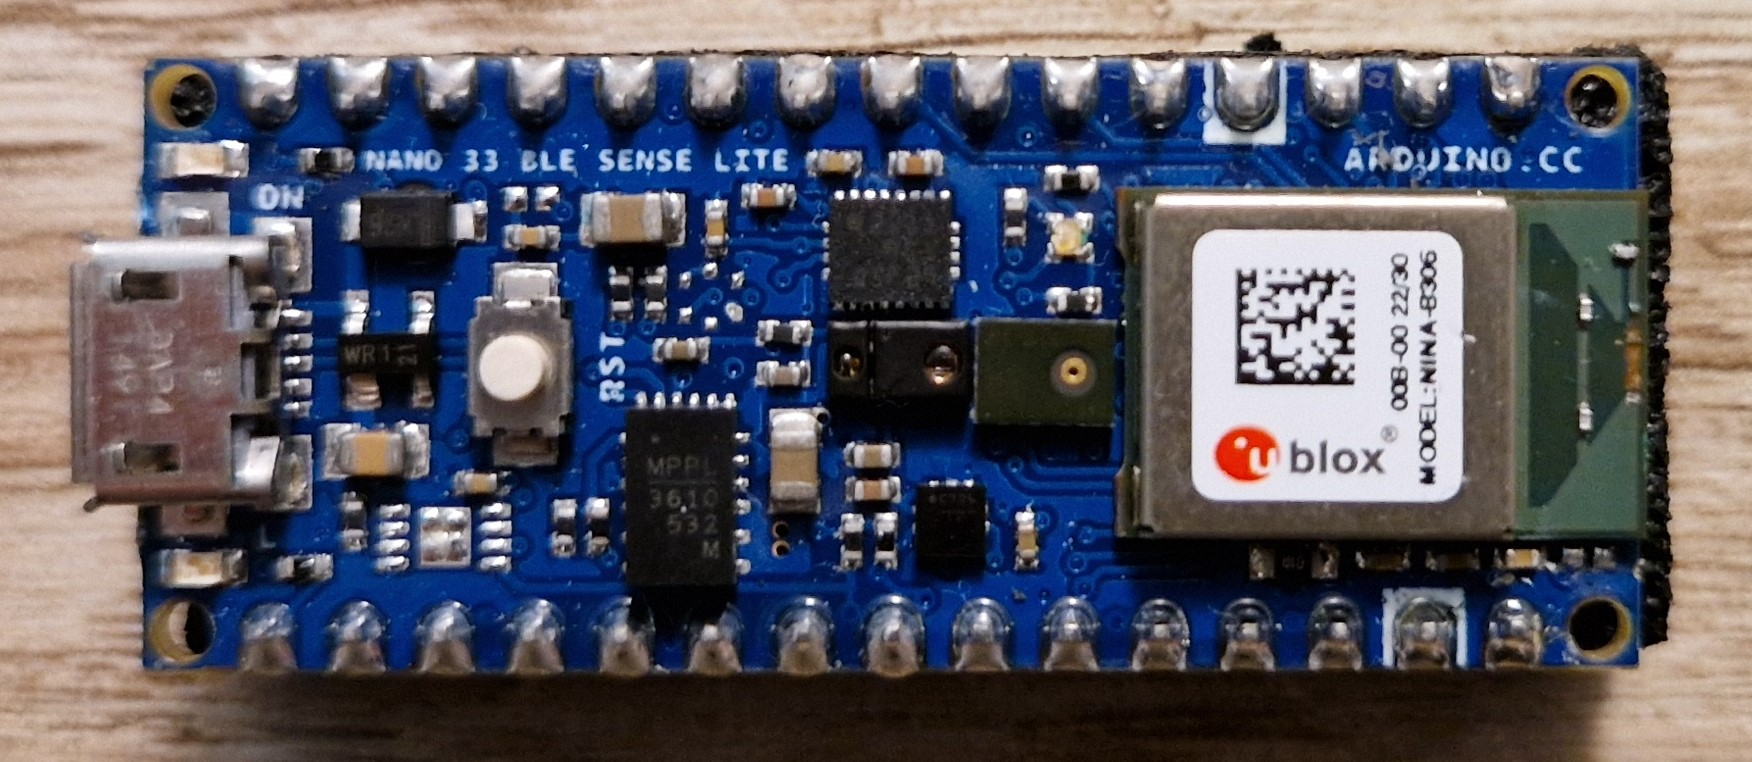
\includegraphics[width=0.7\textwidth]{Images/ArduinoNano33BLESenseLiteTopView}
	\caption{Arduino Nano 33 BLE Sense Lite Top View}
	\label{fig:Arduino Nano 33 BLE Sense Lite}
\end{figure}

	\section{Differences Between Arduino Nano 33 BLE Sense Rev1, Rev2, and Lite}
	
	The Tiny Machine Learning Kit includes only the Arduino Nano 33 BLE Sense Lite. The following outlines the differences between the three different versions.
	
	The differences between the Arduino Nano 33 BLE Sense Rev1 and Arduino Nano 33 BLE Sense Rev2 pertain to the IMU, temperature and humidity sensor, microphone, crypto chip, and voltage regulator. In the second revision, the IMU LSM9DS1 was replaced with two modules: the BMI270 (accelerometer and gyroscope) and the BMI150 (magnetometer). Regarding humidity sensors, the Arduino Nano 33 BLE Sense includes the HTS221 humidity and temperature sensor, while the Arduino Nano 33 BLE Sense Rev2 replaces it with the HS3003 sensor, which promises higher accuracy. Despite the change from the MP34DT05 microphone to the MP34DT06JTR, the microphone specifications remain unchanged. Similarly, only the component names differ for the voltage regulators. The first-generation board uses the MPM3610, while Rev2 employs the MP2322. However, the crypto chip has been removed in Rev2.
	
	The Arduino Nano 33 BLE Sense Lite differs only slightly from the Arduino Nano 33 BLE Sense. The only difference between the two models is that the Lite version does not include the HTS221 but instead features the LPS22HB sensor. This sensor is a pressure sensor but can also measure temperature. However, it cannot measure humidity. To measure relative humidity, an external sensor must be connected. The reason for this decision is that the Arduino company has faced difficulties in maintaining sufficient inventory. \cite{ArduinoForum2023}.
	
\section{On-board Sensors Description}

	
	\section{Arduino Nano 33 BLE Sense: Features and Specifications}
	
	The Arduino Nano 33 BLE Sense is a compact, low-power microcontroller board, ideal for Internet of Things (IoT) and Artificial Intelligence (AI) applications, where space and power efficiency are critical. Measuring only 45mm \( \times \) 18mm, the board operates on 3.3V and includes embedded sensors that make it versatile for practical applications without requiring additional circuitry \cite{ArduinoNano33Sense2025}. 
	
	\subsection{Embedded Sensors}
	
	The board comes equipped with several sensors for data acquisition, including:
	\begin{figure}[h]
		\centering
		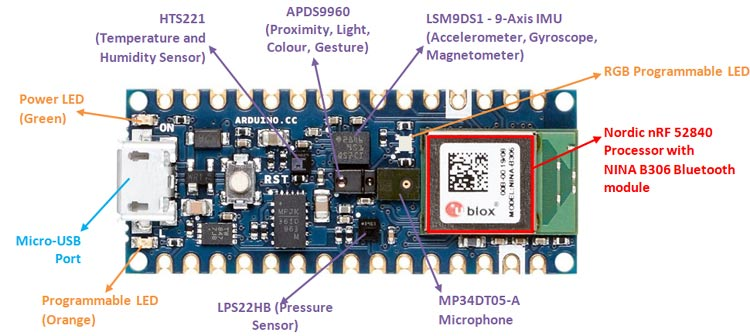
\includegraphics[width=0.7\textwidth]{Images/ArduinoNano33BLESenseHardwareOverview}
		\caption{Components in Arduino Nano 33 BLE Sense}
		\label{fig:Components in Arduino Nano 33 BLE Sense}
	\end{figure}
	\begin{itemize}
		\item \textbf{LSM9DS1 (IMU):} A 9-axis Inertial Measurement Unit (IMU) combining a 3D accelerometer, gyroscope, and magnetometer. It detects orientation, motion, and vibrations, making it suitable for wearable devices \cite{Alushi2024}.
		\item \textbf{APDS-9960:} A digital proximity, ambient light, RGB, and gesture sensor. It can measure proximity distance, detect light levels, and identify colors and gestures \cite{Ava15}.
		\item \textbf{LPS22HB:} A barometric pressure sensor that measures environmental pressure and provides a 24-bit pressure data output. It can also calculate the height above sea level \cite{STM:2017}.
		\item \textbf{HTS221:} A capacitive digital sensor that measures relative humidity and temperature with high accuracy. Its temperature accuracy is ±0.5°C between 15°C and 40°C \cite{STM23}.
		\item \textbf{MP34DT05:} A digital microphone that enables real-time sound capture and analysis, which can be used for creating voice interfaces \cite{STM:2021}.
	\end{itemize}
	
	\subsection{Additional Features}
	
	\begin{itemize}
		\item \textbf{USB Port:} Allows connection to a computer for power supply, data transfer, and serial communication.
		\item \textbf{LEDs:} Three LEDs are available on the board: an RGB programmable LED, a built-in orange programmable LED, and a power LED.
		\item \textbf{Standard Communication Protocols:} Supports UART, I2C, and SPI, enabling interaction with external circuits and sensors for data transfer.
	\end{itemize}
	
	\subsection{Technical Specifications}
	
	The Arduino Nano 33 BLE Sense features a powerful nRF52840 microcontroller from Nordic Semiconductors, based on a 32-bit ARM\textsuperscript{\textregistered} Cortex\texttrademark-M4 CPU running at 64 MHz. Other key specifications include:
	
	\begin{table}[h!]
		\centering
		\begin{tabular}{|l|l|}
			\hline
			\textbf{Feature}                 & \textbf{Specification} \\
			\hline
			Microcontroller                  & nRF52840                     \\
			Operating Voltage                & 3.3V                        \\
			Input Voltage (Limit)            & 21V                         \\
			DC Current Per I/O Pin           & 15 mA                       \\
			Clock Speed                      & 64 MHz                      \\
			CPU Flash Memory                 & 1 MB                        \\
			SRAM                             & 256 KB                      \\
			LED Built-In                     & Pin 13                      \\
			IMU                              & LSM9DS1                     \\
			Microphone                       & MP34DT05                    \\
			Gesture, Light, Proximity, Colour & APDS-9960                   \\
			Barometric Pressure              & LPS22HB                     \\
			Temperature, Humidity            & HTS221                      \\
			\hline
		\end{tabular}
		\caption{Technical Specifications of Arduino Nano 33 BLE Sense \cite{ArduinoNano33Sense2025}}
	\end{table}
	
	\subsection{Important Notes}
	
	\begin{itemize}
		\item \textbf{Voltage Limitations:} Never apply more than 3.3V to the pins, as higher voltages can damage the board .
		\item \textbf{Sensor Placement:} Proper placement of sensors in the environment is critical for accurate readings, especially for factors like temperature, humidity, and air pressure.
		\item \textbf{Operating Conditions:} The board operates reliably within a temperature range of -40°C to 85°C.
	\end{itemize}
	
	The Arduino Nano 33 BLE Sense is a versatile, energy-efficient board that supports a wide range of applications, from environmental monitoring to wearable device development. Its combination of embedded sensors, low power consumption, and small size makes it an ideal choice for modern IoT and AI projects.\cite{ArduinoNano33Sense2025}
	



